\chapter{Introduction}

When I began my PhD, the field of language modeling was already in the midst of rapid change. In 2021, the release of GPT-3—with its \textbf{175 billion parameters}—felt like a watershed moment, a leap that brought artificial systems closer to the scale of biological intelligence. The comparison to the \textbf{86 billion neurons} in the adult human brain \citep{azevedo2009neurons} was irresistible. To many, this parallel symbolized the astonishing pace at which artificial systems appeared to be encroaching on biological complexity.

Yet in the short span of four years, that sense of awe has been recontextualized. \textbf{GPT-4}, though not officially disclosed, is widely estimated to contain \textbf{around 1.8 trillion parameters}, while Google's \textbf{Gemini Ultra} has been reported at roughly \textbf{1.5 trillion}. These figures mark an \emph{order-of-magnitude leap} from GPT-3 and reflect a broader trend: the frontier of large-scale language models is rapidly expanding—both in scale and in sophistication.

This expansion has been accompanied by clear gains in capability. Tasks once viewed as aspirational—such as reasoning over long contexts \citep{lewis2020retrieval}, synthesizing code \citep{chen2021evaluating}, or interpreting multi-step instructions \citep{wei2022chain}—have become tractable for these large models. Performance is typically benchmarked on standard evaluations like MMLU \citep{hendrycks2021mmlu}, BIG-bench \citep{srivastava2023bigbench}, and HellaSwag \citep{zellers2019hellaswag}, where state-of-the-art models have seen rapid gains since 2021.

This \emph{order-of-magnitude leap} in the size of language models raises a fundamental question: \textbf{Are we building better language models, or simply bigger ones?}

This question becomes particularly salient when we examine model performance over time. As \cref{fig:model_size_vs_performance} demonstrates, there's a striking divergence in the language modeling landscape. While large models (\textbf{\textcolor[HTML]{A0DDFF}{blue} line}) show consistent improvement year after year, smaller models of fixed size (\textbf{\textcolor[HTML]{C1CEFE}{purple} line}, ~100M parameters) have plateaued despite advances in training techniques. This trend suggests that our progress may be more about scaling than about fundamental advances in efficiency.

\begin{figure}[htbp]
    \centering
    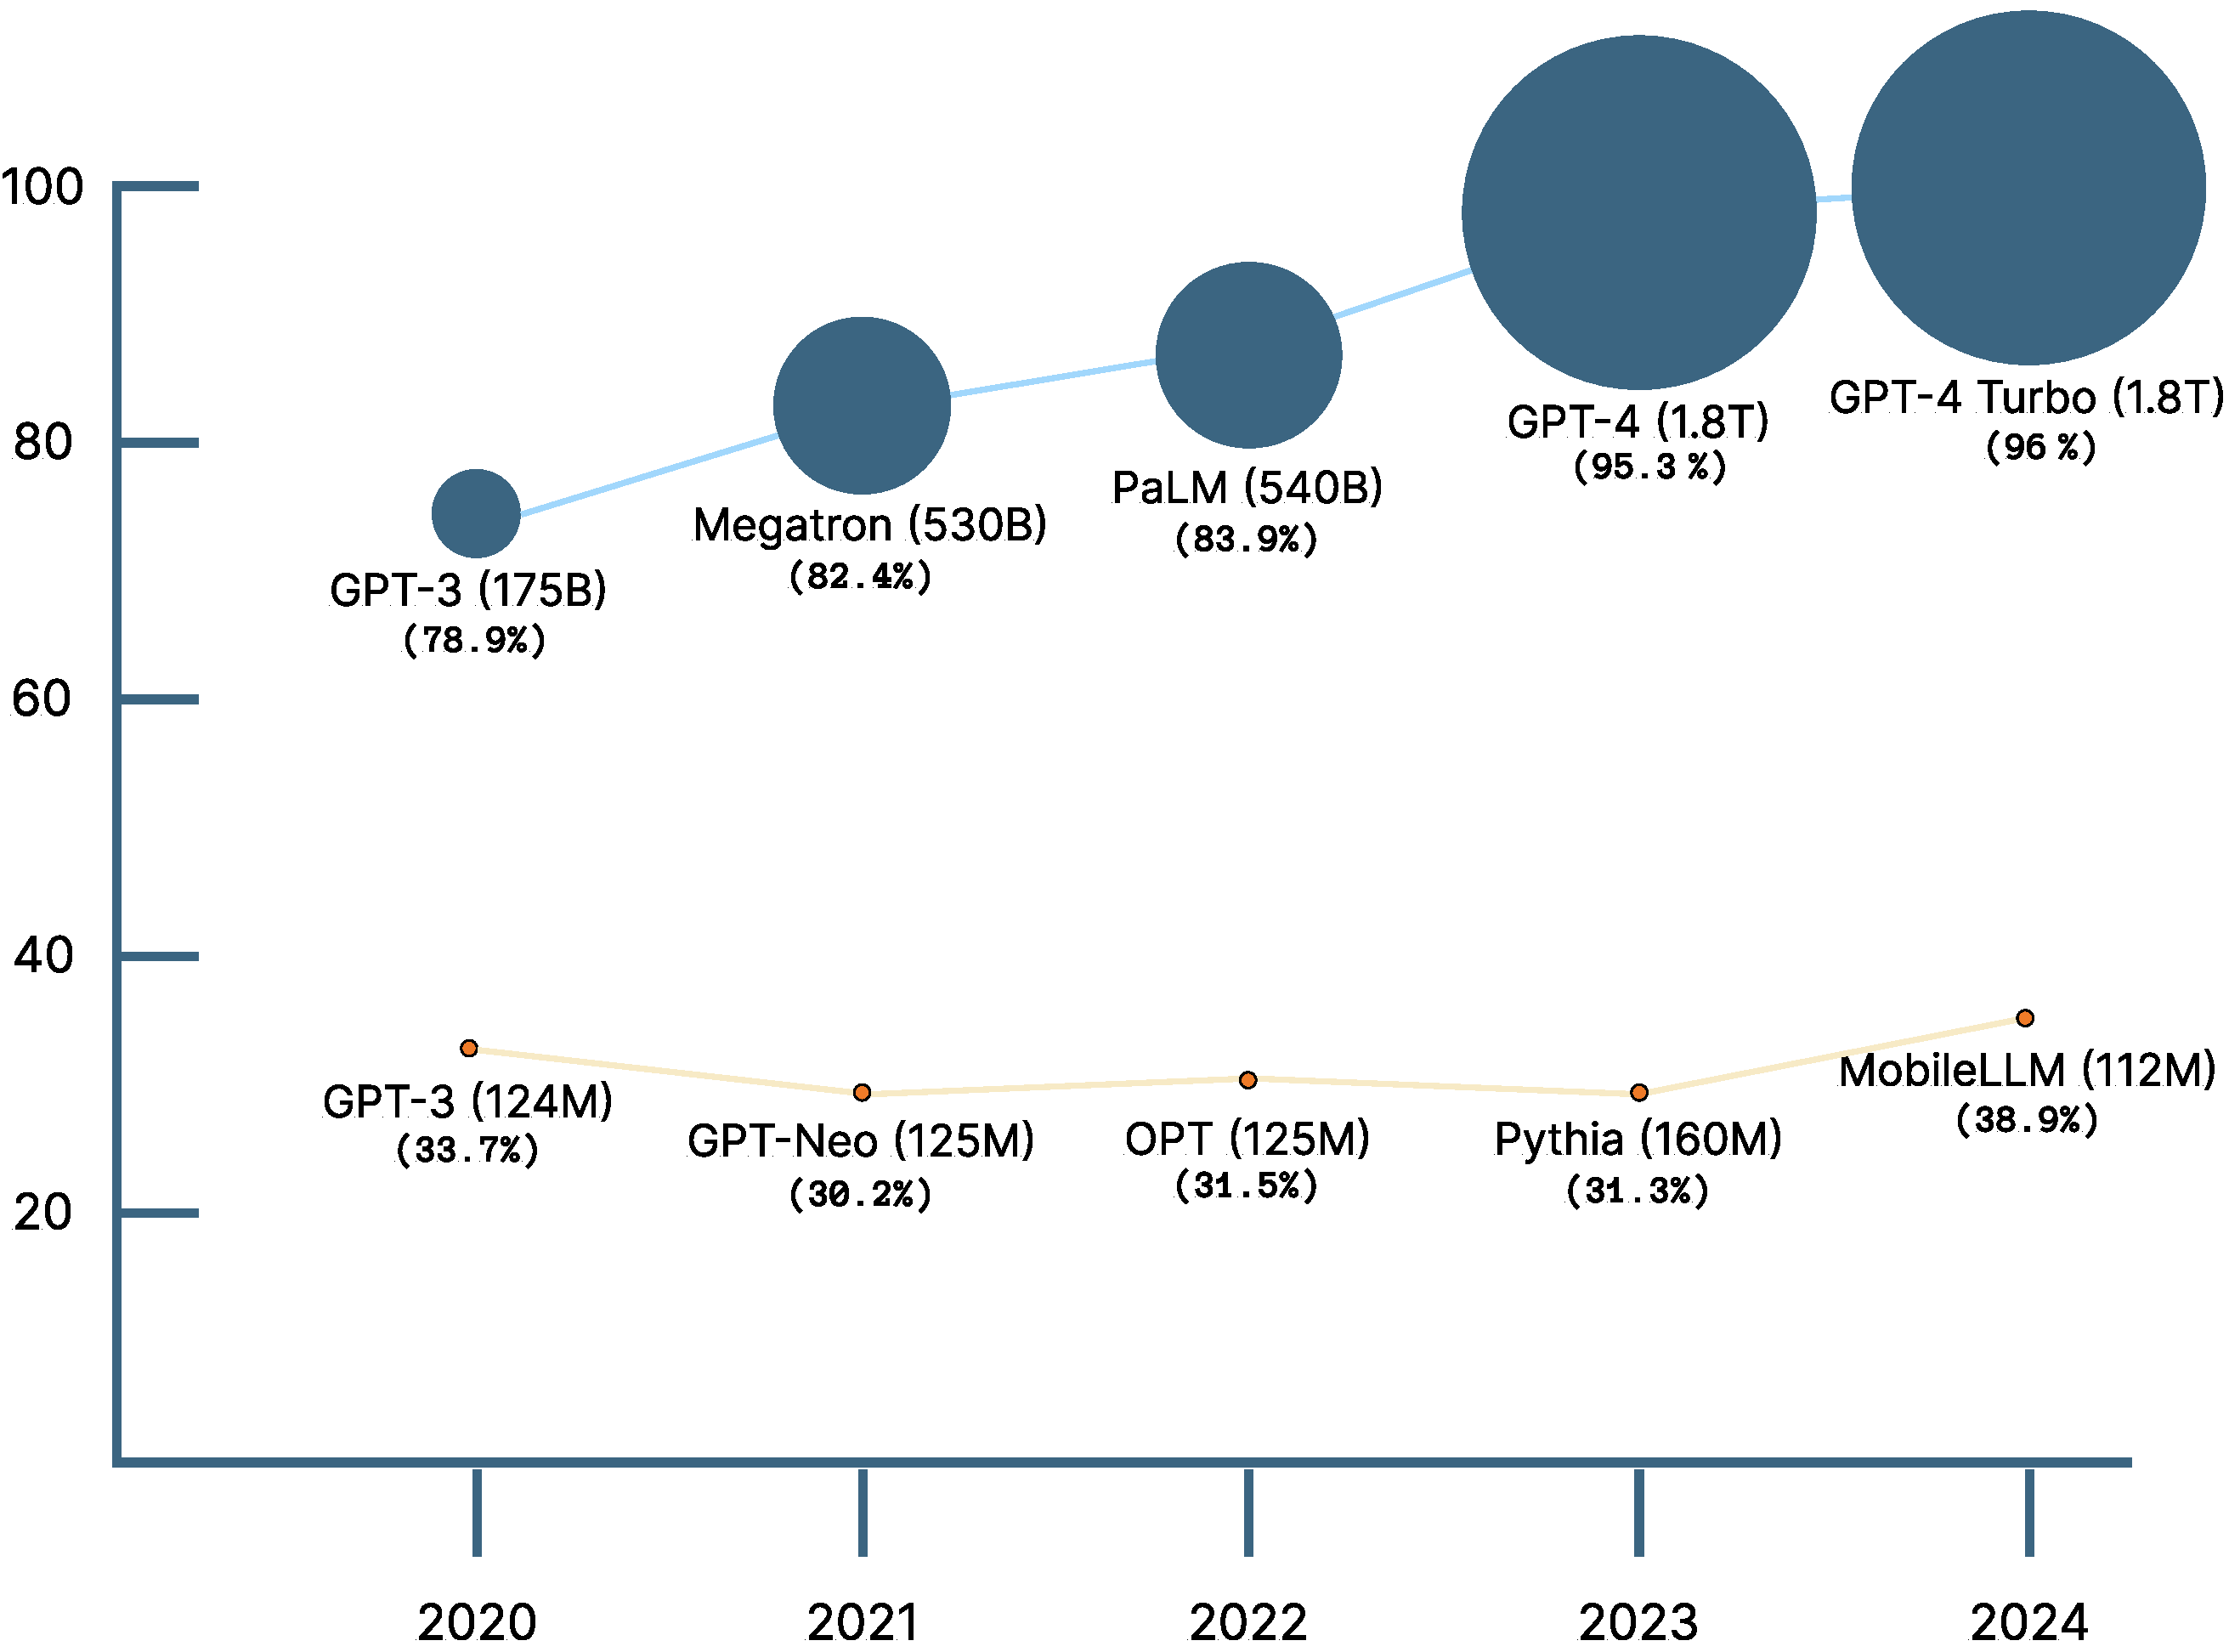
\includegraphics[width=0.8\textwidth]{chapters/introduction/figures/lm_performance_comparison.pdf}
    \caption{Performance of small and large language models on the HellaSwag dataset over time. The plot reveals a striking divergence: while large models (blue) show consistent improvement, smaller models (red) have plateaued despite advances in training techniques.}
    \label{fig:model_size_vs_performance}
\end{figure}

This question is particularly pressing because, while large models continue to push boundaries, \textbf{small models remain essential} for practical deployment. 

\section{Why Do Small Models Matter?}

The rapid scaling of language models has brought about remarkable capabilities, but it has also surfaced a host of challenges and risks \citep{bommasani2021foundation}. Tiny language models—compact, efficient, and accessible—offer a promising path to address many of these issues.

\paragraph{Large foundation models, as discussed by \citet{bommasani2021foundation}, introduce significant societal risks.} These include the potential for generating disinformation and misinformation at scale, amplifying biases and discrimination present in training data, and memorizing and regurgitating sensitive or copyrighted content. The sheer scale of these models also raises concerns about labor displacement, environmental impact, and the creation of single points of failure—where a widely deployed model, if compromised, could have cascading negative effects across all downstream applications. Notably, the authors highlight that the risks associated with large models are not just technical but also social, as they can entrench power in the hands of a few organizations and make it harder to adapt models to specific, local needs.

\paragraph{Environmental sustainability is another critical concern.} The community has been urged to treat energy efficiency as a first-class evaluation metric alongside accuracy \citep{schwartz2020greenai}. Studies have quantified the financial and carbon costs of training state-of-the-art NLP systems, revealing orders-of-magnitude differences between large and compact models \citep{strubell2019energy}. For example, a modest increase in translation accuracy can result in a dramatic rise in compute cost. Tools like the ML Emissions Calculator \citep{lacoste2019quantifying} and systematic reviews of emissions factors \citep{luccioni2023counting} have made it clear that model size, hardware, and training recipes all play a role in determining the environmental footprint of machine learning. Transformer-based models, in particular, are among the most energy-intensive, especially when techniques like neural architecture search are used. Benchmarks such as HULK \citep{zhou2021hulk} have compared pretrained models’ energy efficiency, showing that smaller models are far more efficient in both time and cost. Furthermore, the location where models are trained can significantly affect emissions, and sparsely activated models can be much more energy-efficient than their dense counterparts \citep{patterson2021carbon}. The overall trend is clear: smaller models are more sustainable, and their adoption is crucial for reducing AI's environmental impact.

\paragraph{Data privacy and memorization risks are also heightened in large models.} Research has shown that neural networks, especially large ones, can memorize and regurgitate rare or sensitive training data \citep{feldman2020neural, carlini2019secret}. Follow-up studies have demonstrated that memorization increases with model size and data duplication, and have introduced methods to extract such memorized content from models without access to the original training set \citep{carlini2021extracting, carlini2022quantifying}. Comprehensive surveys have categorized the security and privacy risks of large language models, including inference-time leakage, adversarial vulnerabilities, and systemic risks from centralization \citep{yao2024privacysurvey}. Larger models are more likely to leak personally identifiable information, especially when trained on duplicated or low-diversity data \citep{huang2022large, neel2023privacy}. Mitigation strategies such as differential privacy \citep{dwork2006calibrating} and federated learning \citep{mcmahan2017communication} have been proposed, but these often come with trade-offs in model utility. Scaling laws for memorization further confirm that as models grow, so does their propensity to memorize and leak sensitive information \citep{lu2024scaling, biderman2023emergent, kiyomaru2024comprehensive}. In contrast, smaller models, with less capacity to memorize, offer a more privacy-preserving alternative—especially when combined with privacy-focused training techniques.

\paragraph{Tiny models are also uniquely suited for on-device and edge deployment.} Efficient inference with limited memory is essential for running language models on consumer hardware, and recent work has shown that even models with billions of parameters can be optimized for such use cases \citep{alizadeh2024llm}. Sub-billion parameter models are particularly important for energy-efficient, on-device applications, as demonstrated by \citet{liu2024mobilellm}. Earlier advances in mobile-friendly architectures, such as MobileNets \citep{howard2017mobilenets} and EfficientFormer \citep{li2022efficientformer}, laid the groundwork for efficient models in both vision and language domains. The importance of energy-proportional memory for datacenter and mobile applications has also been highlighted \citep{malladi2012towards}. These advances make it possible to run language models in privacy-sensitive, resource-constrained, or offline settings, broadening the reach and utility of AI.

\paragraph{Interpretability and scientific understanding are further reasons to prioritize small models.} The internal mechanisms of transformers and other neural architectures are more tractable in smaller models, making them better testbeds for developing scientific understanding \citep{elhage2021mathematical, elhage2022toy, bircken2023monosemanticity, anthropic2023components}. Tools such as influence functions are easier to apply at small scale, and the “manifold hypothesis” suggests that smaller models are ideal for probing the structure of neural representations \citep{olah2014manifolds}. Progress in understanding larger models often begins with insights gained from studying their smaller counterparts.

\paragraph{Finally, the democratization and accessibility of language technology depend on the availability of small, open models.} The cost of training and deploying large models is rising rapidly, with the financial and hardware requirements putting them out of reach for most organizations and individuals \citep{cottier2024rising, sharir2020cost}. Minimal, well-documented implementations like nanoGPT \citep{karpathy2023nanogpt} and Pico \citep{diehlmartinez2025pico} make language modeling accessible to a broader community, supporting education, experimentation, and innovation. By lowering the barrier to entry, small models enable more researchers, organizations, and communities to participate in the development and application of language technologies.

In summary, tiny language models matter because they are more sustainable, privacy-preserving, interpretable, and accessible. They offer a practical and ethical path forward for language technology, especially as the risks and costs of large-scale models continue to mount.

\section*{Research Objectives}

This thesis aims to explore how small language models can be trained more efficiently and effectively, emphasizing principled approaches over brute-force scaling. The work is structured around two central research objectives:

\subsection{Can cognitively-inspired learning paradigms improve small model training?}

Despite recent advances in architecture design and compression techniques, small models continue to lag behind their larger counterparts. Yet they are critical for real-world deployment due to their efficiency, interpretability, and accessibility.

A persistent challenge in this area is that many of the methods proposed to improve small models—ranging from ad hoc architectural tweaks to various forms of regularization or data augmentation—often lack a strong scientific foundation. Progress is frequently incremental and offer to interpret; new techniques sometimes offering only marginal gains or failing to generalize beyond specific benchmarks. Without a principled framework or guiding thesis, it becomes challenging to systematically understand what works, why it works, and how to build on prior results in a cumulative way.

One promising guiding thesis is to look to human language acquisition for inspiration. While today's large language models are trained on billions of tokens, a typical 13-year-old human has been exposed to only around 100 million words. This dramatic discrepancy highlights a key inefficiency in current training paradigms—and suggests an opportunity: by drawing on cognitive science and principles of human language learning, we may uncover more data-efficient strategies for small models.

By studying the principles and processes underlying human learning, we can develop a more coherent framework for evaluating and designing training paradigms for small models. This approach allows us to ask: do the strategies that work well for the human brain also confer benefits to artificial models? Can cognitive science provide a roadmap for more data-efficient, and robust, language modeling?

This part of the thesis investigates two core levers for improving training efficiency:

\textbf{Data-level learning processes:} Can curriculum learning—structured exposure to data based on notions of `difficulty' or `frequency'—help small models generalize more effectively?

\textbf{Objective-level learning processes:} How can modifying the learning objective or inductive biases (e.g., through syntactic generalization or smoothing) enhance model robustness and reduce reliance on token frequency and instead focus on robust syntactic generalization?

These questions guide an exploration of cognitively inspired approaches to learning, with a focus on grounding small model training in data-efficient, human-aligned paradigms.

\subsection{How can we more quantitatively understand the performance of small models?}

Improving training efficiency is only half the challenge. To ensure scientific progress, we must also develop rigorous and interpretable methods for evaluating small models. Unlike large models—where scale often masks architectural or algorithmic weaknesses—small models expose the fundamental limits of current techniques.

This thesis investigates:

\begin{quote}
    \textbf{\emph{Can we establish more scientific, transparent methods for evaluating and understanding small language models?}}
\end{quote}

Existing benchmarks often reward scale rather than understanding. This work aims to shift the focus toward learning dynamics, convergence behavior, and interpretability—metrics that provide deeper insight into why and how models learn.

By developing diagnostic tools and lightweight frameworks tailored to small models, this thesis contributes to a more empirical, reproducible, and theory-grounded methodology for language modeling research.

\section*{Thesis Overview}

This thesis is organized into two parts, reflecting the two research threads:

\subsection*{Part I: Cognitive Insights for Efficient Training (Chapters 2–4)}

\begin{itemize}

    \item \textbf{Chapter 2:} \emph{Language Modeling Background and Small Language Models} provides a background on language modeling, including the early approaches, word embeddings, and language models, leading up to current state of the art large language models. It also outlines some of the methods that researchers have used to make progress on efficiently training small language models.

    \item \textbf{Chapter 3:} \emph{Curriculum Learning for Infant-Inspired Model Building}  
    explores curriculum strategies inspired by human language acquisition, using the BabyLM Challenge's strict 10-million-word cap as a testbed for evaluating data-efficient learning.

    \item \textbf{Chapter 4:} \emph{Mitigating Frequency Bias and Anisotropy in Language Model Pre-Training with Syntactic Smoothing}  
    introduces a novel technique to improve the representation of infrequent tokens by distributing learning signals through syntactic similarity, reducing reliance on frequency and improving robustness.
\end{itemize}

\subsection*{Part II: An Analytical Lens on Learning Dynamics (Chapters 5–7)}

\begin{itemize}
    \item \textbf{Chapter 5:} \emph{Model Analysis Background} provides a background on the methods used to analyze language models, including activation patterns, parameter rank, and convergence behavior.

    \item \textbf{Chapter 6:} \emph{Tending Towards Stability: Convergence Challenges in Small Language Models}  
    investigates why small models often saturate during training. Using the Pythia model suite, it analyzes activation patterns, parameter rank, and convergence behavior.

    \item \textbf{Chapter 7:} \emph{Pico: A Lightweight Framework for Studying Language Model Learning Dynamics}  
    presents Pico, a modular framework for transparent training and in-depth analysis of learning dynamics, enabling reproducible experiments with small models.
\end{itemize}

\section*{Contributions}

This work contributes to the field by:

\begin{enumerate}
    \item Exploring an in-depth analysis of the curriculum learning paradigm from a cognitive perspective.

    \item Introducing novel methods—such as syntactic smoothing and structured curricula—for improving small model generalization.

    \item Developing analysis tools to diagnose and analyze inefficiencies in model training.

    \item Construction of an open-source framework for studying language model learning dynamics that can inform better training methods.
\end{enumerate}

Together, these contributions aim to support a more \textbf{accessible, efficient, and sustainable future} for language modeling—particularly for researchers and developers working under real-world constraints.
